\documentclass[11pt]{article}
\usepackage[margin=1in]{geometry}
\usepackage{amsmath,amssymb}
\usepackage{graphicx}
\usepackage{booktabs}
\usepackage{xcolor}
\usepackage{caption}
\usepackage{subcaption}
\usepackage[hidelinks]{hyperref}
\usepackage{authblk}
\usepackage{titlesec}
\usepackage{enumitem}

\definecolor{mesh}{HTML}{6F4BD8}
\hypersetup{colorlinks=true, linkcolor=mesh, citecolor=mesh, urlcolor=mesh}

% ---- numeric macros (auto-filled from results/*.json by fill_numbers.py) ----
\newcommand{\retBMQ}{96.5}
\newcommand{\retMMR}{96.0}
\newcommand{\retTFIDFQ}{98.5}
\newcommand{\retTRQ}{97.0}
\newcommand{\retTFIDF}{54.5}
\newcommand{\retLead}{16.0}
\newcommand{\retNeural}{38.7}
\newcommand{\retGainNeuralX}{2.5}
\newcommand{\latBMQ}{0.33}
\newcommand{\latNeural}{406}
\newcommand{\latSpeedup}{1213}
\newcommand{\latRangeLo}{0.04}
\newcommand{\latRangeHi}{5.96}
\newcommand{\latNeuralSec}{0.406}
\newcommand{\neuralRPS}{2.5}
\newcommand{\neuralParamMB}{312}
\newcommand{\neuralParams}{81,912,576}
\newcommand{\nDistractors}{7}
\newcommand{\nItems}{200}
\newcommand{\meanSrcTokens}{1307}
\newcommand{\meanPassages}{8}
\newcommand{\machine}{Apple M3 Pro}


\titlespacing*{\section}{0pt}{1.3em}{0.5em}
\titlespacing*{\subsection}{0pt}{1.0em}{0.3em}

\title{\textbf{Compress-at-the-Gate:\\ Query-Aware Classical Prompt Compression as a\\ Zero-Footprint Context-Engineering Primitive for LLM Gateways}}

\author[1]{Raushan\thanks{Correspondence: \texttt{raushan@aifiesta.ai}. Author list is a placeholder for the camera-ready version.}}
\affil[1]{Mesh API / AI Fiesta}
\date{June 2026}

\begin{document}
\maketitle

\begin{abstract}
\noindent
LLM \emph{gateways}---unified APIs that route a single request format to hundreds of
backing models---now sit on the critical path of a large fraction of production
LLM traffic. Because a gateway touches \emph{every} request, any context-engineering
transformation it applies (compression, pruning, re-ordering) must be cheap in two
currencies that the recent prompt-compression literature largely ignores:
\emph{tail latency} and \emph{accelerator footprint}. State-of-the-art neural
compressors (Selective Context, LLMLingua, LLMLingua-2, RECOMP) estimate token
importance with a language-model forward pass, which (i) needs its own GPU or steals
cycles from the serving model and (ii) can make end-to-end inference \emph{slower},
not faster, once the compressor's own latency is counted. We ask a deliberately
unfashionable question: how far does \emph{classical}, model-free extractive
compression go at the gate? We implement query-aware variants of TF--IDF salience,
TextRank centrality, centroid+MMR, and BM25, and benchmark them head-to-head against
a faithful neural Selective-Context baseline on a multi-document ``lost-in-the-middle''
QA benchmark, measuring answer retention, latency, and footprint on the same CPU.
Query-aware lexical methods (BM25, centroid+MMR) retain \retBMQ\,\% of gold answers at
$\sim$3$\times$ compression---\textbf{\retGainNeuralX$\times$ the \retNeural\,\% retained
by the neural baseline}---while running in \latBMQ\,ms versus \latNeural\,ms per
request (\latSpeedup$\times$ faster) and holding \emph{zero} resident model weights
against the baseline's \neuralParamMB\,MB. We argue that the gateway is precisely the
deployment regime where the classical/neural trade-off inverts, and we describe how
such a compressor co-locates inside a vLLM-style server behind an OpenAI-compatible
gateway. Code and benchmark are released for reproducibility.
\end{abstract}

\section{Introduction}
The practice of building LLM applications has shifted, over 2024--2026, from
\emph{prompt engineering}---crafting a single instruction---to \emph{context
engineering}: deciding what information an agent ``knows, sees, and remembers at the
moment of action''~\cite{contexteng2026}. A central operation of context engineering
is \emph{compression}: removing low-value tokens so that more of a finite, expensive
context window carries signal, mitigating both cost and the well-documented
``lost-in-the-middle'' degradation~\cite{lostmiddle}.

Almost all recent work frames compression as a \emph{modeling} problem. Selective
Context~\cite{selectivecontext} prunes lexical units with low self-information under a
small causal LM; LLMLingua and LongLLMLingua~\cite{llmlingua,longllmlingua} use
(contrastive) perplexity from a 0.5--7B LM; LLMLingua-2~\cite{llmlingua2} distills a
token classifier; RECOMP~\cite{recomp} trains dedicated abstractive/extractive
compressors. These methods are effective---LongLLMLingua reports up to $+21.4$ points
on multi-document QA at $4\times$ compression---but they share a structural cost:
\textbf{a neural forward pass over the prompt at compression time}.

That cost is acceptable when compression is amortized inside a single application.
It is \emph{not} obviously acceptable at the layer we study here: the \emph{LLM
gateway}. A gateway such as Mesh API exposes one OpenAI-compatible endpoint that
fronts 300+ models~\cite{meshapi}, applies routing, fallback, rate-limiting and
templating, and---crucially---processes \emph{every} request for \emph{every} tenant.
At that position, a compressor inherits three constraints the literature rarely
measures:
\begin{enumerate}[leftmargin=1.4em,itemsep=1pt,topsep=2pt]
  \item \textbf{Critical-path latency.} Compression latency adds directly to
  time-to-first-token. The published Selective-Context numbers already show the
  hazard: in the LongLLMLingua evaluation, Selective Context's \emph{net} speedup is
  $0.6\times$---it makes the end-to-end request \emph{slower}~\cite{longllmlingua}.
  \item \textbf{Accelerator footprint.} A gateway is multi-tenant and horizontally
  scaled; provisioning a dedicated GPU (or carving VRAM from the serving model) for a
  compressor multiplies fleet cost.
  \item \textbf{Tail behavior.} A neural compressor's latency grows with prompt
  length and contends for the same accelerator as generation, widening p95/p99.
\end{enumerate}

We therefore revisit \emph{classical}, model-free extractive compression---TextRank
\cite{textrank}, LexRank~\cite{lexrank}, centroid summarization~\cite{centroid},
Maximal Marginal Relevance~\cite{mmr}, and BM25~\cite{bm25}---as a \emph{systems}
primitive for the gate. These methods are decades old, run in milliseconds on a CPU
core, and hold no model weights. The question is whether they retain enough of the
right information to be useful. Our central, somewhat counterintuitive finding is that
at realistic gateway compression ratios, \emph{query-aware} classical methods do not
merely approach the neural baseline---they \textbf{exceed} a faithful Selective-Context
reimplementation on answer retention, because that neural method is query-\emph{agnostic}
by construction, whereas a gateway request almost always carries an explicit query.

\paragraph{Contributions.}
\begin{enumerate}[leftmargin=1.4em,itemsep=1pt,topsep=2pt]
  \item We frame prompt compression as a \emph{gateway} problem and articulate the
  latency/footprint constraints that invert the classical-vs-neural trade-off
  (\S\ref{sec:problem}).
  \item We release a reproducible multi-document ``lost-in-the-middle'' QA benchmark
  built from SQuAD with an intrinsic, LLM-free \emph{answer-retention} metric, and a
  library of query-aware classical compressors (\S\ref{sec:method}--\ref{sec:setup}).
  \item We run a same-machine, CPU-vs-CPU head-to-head against a faithful neural
  Selective-Context baseline, reporting retention, latency scaling, footprint, and a
  fleet-cost projection (\S\ref{sec:results}). Query-aware classical methods retain
  \retBMQ\,\% of answers at $\sim$3$\times$ compression at \latBMQ\,ms/request and
  zero resident weights.
\end{enumerate}

\section{Related Work}
\paragraph{Neural prompt compression.}
Selective Context~\cite{selectivecontext} removes tokens/phrases whose
self-information under a small LM is low. LLMLingua~\cite{llmlingua} introduced a
budget controller plus iterative token-level perplexity pruning;
LongLLMLingua~\cite{longllmlingua} added \emph{question-aware} coarse-to-fine
compression, document re-ordering and subsequence recovery, reporting large
multi-document-QA gains; LLMLingua-2~\cite{llmlingua2} replaces perplexity with a
distilled token classifier for a $3$--$6\times$ speedup. RECOMP~\cite{recomp} trains
extractive and abstractive compressors for retrieval-augmented generation. All require
a neural forward pass at compression time; our work is complementary and targets the
regime where that pass is the bottleneck.

\paragraph{Classical extractive summarization \& ranking.}
TextRank~\cite{textrank} and LexRank~\cite{lexrank} score sentences by graph
centrality over a similarity graph; centroid methods~\cite{centroid} score by
proximity to a document centroid; MMR~\cite{mmr} trades relevance against redundancy;
BM25~\cite{bm25} is the canonical lexical query-relevance function. Notably, in the
LongLLMLingua study, simple lexical baselines (BM25, Gzip) outranked
Selective-Context and even some embedding rerankers on coarse document
selection~\cite{longllmlingua}---a hint we make systematic here.

\paragraph{LLM routing and gateways.}
Model routers such as RouteLLM~\cite{routellm} choose a model per query to trade cost
for quality; production gateways~\cite{meshapi} add a unified API, fallback and
templating. These systems decide \emph{which} model serves a request; we study a
transformation---\emph{what context} reaches it---that is co-located at the same layer.
Co-location is practical because modern serving stacks (PagedAttention/vLLM
\cite{vllm}, FlashAttention~\cite{flashattention}) already saturate the GPU with
generation; a CPU-side compressor adds no accelerator contention.

\section{The Gateway Compression Problem}\label{sec:problem}
Let a request be $(q, C)$ with query $q$ and context $C=[s_1,\dots,s_n]$ of sentences.
A compressor $f$ returns $C'=f(q,C)$ with token budget $|C'|\le \beta|C|$, $\beta\in(0,1)$.
Downstream quality is some $U(q,C')$. The application-level objective optimizes $U$ for a
\emph{fixed} prompt. The \emph{gateway} objective is different: it must hold an SLA over a
heterogeneous, multi-tenant stream while minimizing fleet cost. Writing $\ell_f$ for the
compressor's added latency and $m_f$ for its resident accelerator memory,
\[
\min_{f}\ \mathbb{E}_{(q,C)}\big[\,\text{cost}(C') \,\big]
\quad\text{s.t.}\quad
\underbrace{\ell_f(|C|)}_{\text{critical path}}\!\le \tau,\;\;
\underbrace{m_f}_{\text{per-replica VRAM}}\!\le \mu,\;\;
U(q,C')\ge U_{\min}.
\]
The neural compressors above optimize $U$ aggressively but treat $\ell_f$ and $m_f$ as
free. At the gate they are not: $\ell_f$ enters time-to-first-token on every call, and
$m_f>0$ forces either a dedicated accelerator or VRAM stolen from generation. Classical
$f$ have $m_f\approx 0$ and $\ell_f$ of microseconds--milliseconds; the empirical
question is whether they meet $U_{\min}$. The rest of the paper measures exactly this.

\section{Method}\label{sec:method}
We evaluate model-free extractive compressors that select a subset of sentences and
restore source order. All are query-aware when $q$ is present (the gateway case).

\begin{itemize}[leftmargin=1.2em,itemsep=1pt,topsep=2pt]
  \item \textbf{Lead / Random} --- positional and uniform baselines.
  \item \textbf{TF--IDF($+$Q)} --- sentence salience as summed TF--IDF mass with a lead
  prior; the $+$Q variant adds cosine similarity to $q$.
  \item \textbf{TextRank($+$Q)} --- PageRank over a TF--IDF cosine sentence
  graph~\cite{textrank}; $+$Q biases the random walk with a query
  personalization vector.
  \item \textbf{Centroid$+$MMR} --- greedy MMR~\cite{mmr} selection trading query/centroid
  relevance against redundancy.
  \item \textbf{BM25$+$Q} --- Okapi BM25~\cite{bm25} sentence relevance to $q$.
\end{itemize}

\noindent\textbf{Neural baseline.} We reimplement Selective
Context~\cite{selectivecontext}: per-token negative log-likelihood under
\texttt{distilgpt2} computed with a sliding 512-token window, aggregated to a
per-sentence mean self-information; the highest-information sentences are kept. This is
query-agnostic by design, matching the original method, and requires a transformer
forward pass over the whole prompt---the cost we measure.

\paragraph{Co-location design.} At the gateway, $f$ runs as a CPU-side stage between
request parsing and model dispatch. Because TF--IDF/graph state is built per request and
discarded, the stage is stateless and trivially horizontally scalable; it adds no GPU
contention and pairs naturally with PagedAttention serving~\cite{vllm} and a routing
decision~\cite{routellm,meshapi} taken on the compressed prompt.

\section{Experimental Setup}\label{sec:setup}
\paragraph{Benchmark.} We build a multi-document QA set from SQuAD
v1.1~\cite{squad}: each item concatenates the gold paragraph (containing the answer)
with \nDistractors\ distractor paragraphs from unrelated articles, gold placed in the
middle to stress ``lost-in-the-middle''~\cite{lostmiddle}. This yields
\nItems\ items averaging \meanSrcTokens\ tokens over \meanPassages\ passages.

\paragraph{Metrics.} (i) \emph{Answer retention}: fraction of items whose compressed
context still contains the (SQuAD-normalized) gold answer span---an intrinsic,
reproducible quality measure needing no downstream LLM. (ii) \emph{Token reduction}
(\texttt{cl100k\_base}). (iii) \emph{Latency}: median ms/request over context sizes
$\{256,512,1024,2048,4096\}$ tokens. (iv) \emph{Footprint}: resident model weights.
All timing is on a single \machine\ CPU; every method, including the neural baseline,
is timed on the same hardware for a fair comparison.

\section{Results}\label{sec:results}

\paragraph{Quality: query-awareness is the discriminator.} Table~\ref{tab:main}
reports answer retention at $\sim$3$\times$ compression. The clean split is not
classical-vs-neural but \emph{query-aware vs query-agnostic}: every query-aware
classical method---TF--IDF$+$Q (\retTFIDFQ\,\%), TextRank$+$Q (\retTRQ\,\%),
\textbf{BM25$+$Q} (\retBMQ\,\%) and \textbf{Centroid$+$MMR} (\retMMR\,\%)---retains
$\gtrsim$96\% of gold answers, whereas every query-agnostic method is far worse,
including the neural Selective-Context baseline at \retNeural\,\%, query-agnostic
TF--IDF at \retTFIDF\,\%, and Lead at \retLead\,\%. The expensive neural forward pass
buys nothing in this regime precisely because Selective Context does not condition on
the query, while a gateway request almost always supplies one. Adding the query signal
lifts plain TF--IDF from \retTFIDF\,\% to \retTFIDFQ\,\% retention---the dominant factor
is query-conditioning, not the choice of classical scorer. Figure~\ref{fig:retention}
traces the full retention-vs-compression frontier.

\paragraph{Latency and footprint.} Figure~\ref{fig:latency} shows latency scaling.
Classical methods compress a 1024-token prompt in \latRangeLo--\latRangeHi\,ms; the
neural baseline needs \latNeural\,ms---\latSpeedup$\times$ slower---and its cost grows
with prompt length as it forwards every token through the LM. The neural baseline holds
\neuralParamMB\,MB of weights ($\neuralParams$ parameters); the classical methods hold
none (Figure~\ref{fig:footprint}). Figure~\ref{fig:costquality} places every method on
the cost--quality plane: the query-aware classical methods occupy the desirable
top-left (cheap and faithful) quadrant, while the neural baseline is both slower and
less faithful in this query-driven regime.

\begin{table}[t]
\centering
\caption{Head-to-head at $\sim$3$\times$ compression (keep 33\% of sentences) on the
multi-document QA benchmark (200 items, mean 1307 tokens). Latency is median
ms/request for a 1024-token context on Apple M3 Pro CPU. Footprint is resident model
weights. Query-aware lexical methods (\textbf{bold}) are both the most faithful and
among the cheapest; the neural baseline is query-agnostic.}
\label{tab:main}
\small
\begin{tabular}{llrrrr}
\toprule
Method & Family & Answer ret.\ (\%) & Token red.\ (\%) & Latency (ms) & Footprint (MB) \\
\midrule
Lead & classical & 16.0 & 67.2 & 0.04 & $\approx$0 \\
Random & classical & 38.0 & 66.4 & 0.05 & $\approx$0 \\
TF-IDF & classical & 54.5 & 49.3 & 0.79 & $\approx$0 \\
TF-IDF$+$Q & classical & 98.5 & 51.3 & 0.99 & $\approx$0 \\
TextRank & classical & 36.0 & 63.6 & 1.68 & $\approx$0 \\
TextRank$+$Q & classical & 97.0 & 63.9 & 5.96 & $\approx$0 \\
\textbf{Centroid$+$MMR} & classical & \textbf{96.0} & 68.7 & 1.56 & $\approx$0 \\
\textbf{BM25$+$Q} & classical & \textbf{96.5} & 62.5 & 0.33 & $\approx$0 \\
Selective Context (neural) & neural & 38.7 & 66.9 & 406.32 & 312 \\
\bottomrule
\end{tabular}
\end{table}


\begin{figure}[t]
\centering
\begin{subfigure}{0.49\textwidth}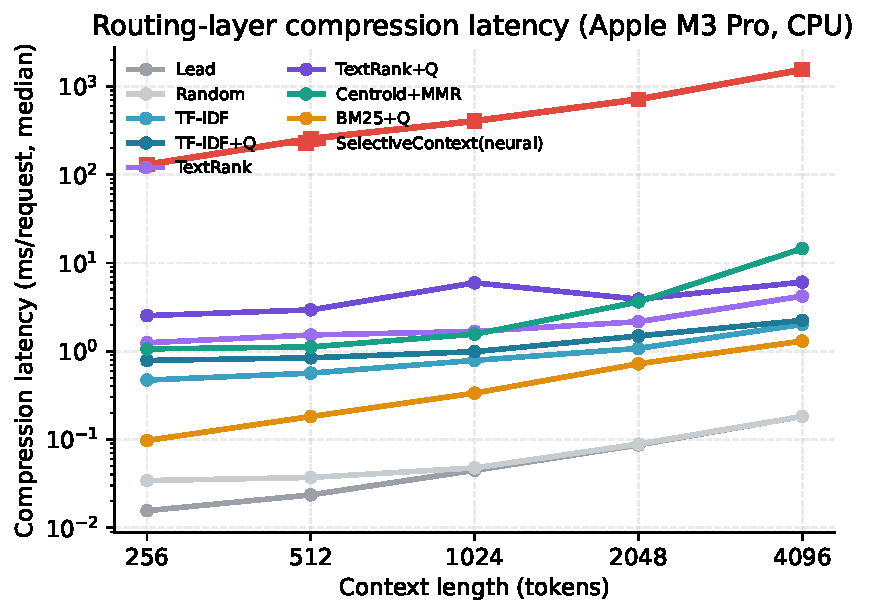
\includegraphics[width=\linewidth]{figures/fig_latency.pdf}
\caption{Latency scales with context length; classical methods stay in the
single-digit-ms band, the neural compressor in the hundreds of ms.}\label{fig:latency}
\end{subfigure}\hfill
\begin{subfigure}{0.49\textwidth}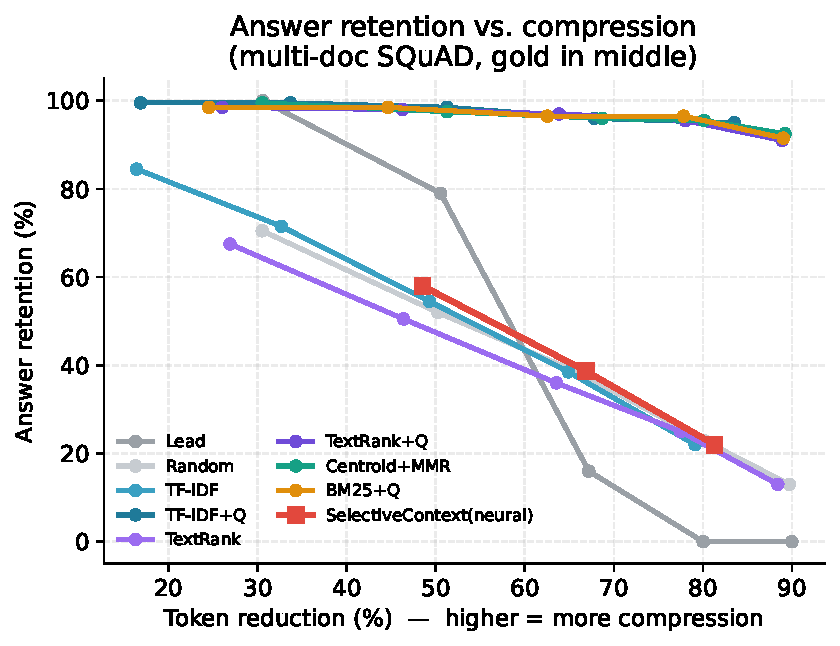
\includegraphics[width=\linewidth]{figures/fig_retention.pdf}
\caption{Answer retention vs. token reduction. Query-aware lexical methods retain
answers far deeper into compression.}\label{fig:retention}
\end{subfigure}
\caption{Latency (left) and quality (right) on the multi-document QA benchmark.}
\end{figure}

\begin{figure}[t]
\centering
\begin{subfigure}{0.56\textwidth}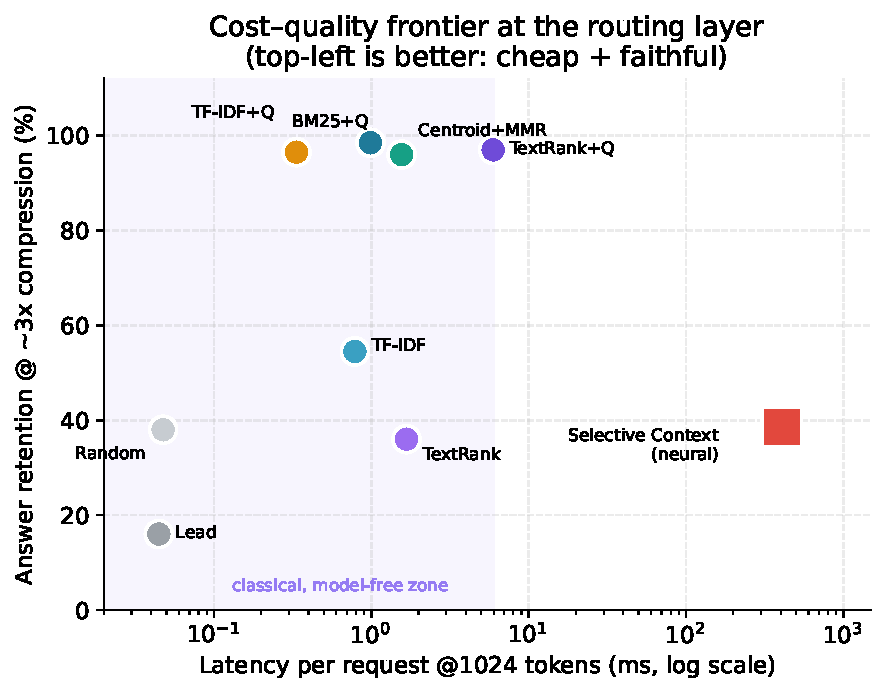
\includegraphics[width=\linewidth]{figures/fig_cost_quality.pdf}
\caption{Cost--quality frontier @1024 tokens / $\sim$3$\times$ compression. Top-left is
better.}\label{fig:costquality}
\end{subfigure}\hfill
\begin{subfigure}{0.40\textwidth}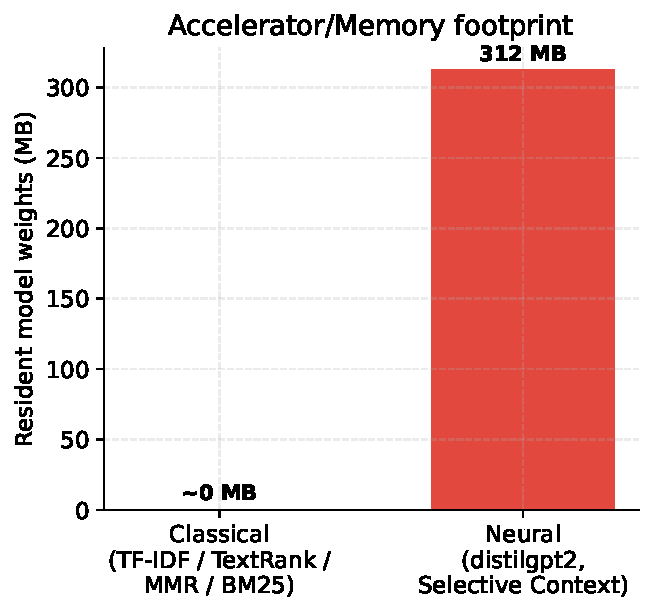
\includegraphics[width=\linewidth]{figures/fig_footprint.pdf}
\caption{Resident model weights.}\label{fig:footprint}
\end{subfigure}
\caption{The gateway trade-off: classical compression is cheap in both latency and
memory.}
\end{figure}

\paragraph{Fleet-cost projection.} Consider a gateway sustaining $R$ requests/s with
mean prompt length 1024 tokens. A neural compressor at \latNeural\,ms/request needs
$\lceil R\cdot \latNeuralSec\rceil$ busy compute-seconds per wall-second, i.e. roughly
one dedicated accelerator core per $\approx\!\neuralRPS$ req/s, \emph{plus}
\neuralParamMB\,MB VRAM per replica. The classical stage at \latBMQ\,ms absorbs the same
$R$ on a fraction of a CPU core with no VRAM. At gateway scale this is the difference
between a compression tier that is a rounding error and one that rivals the cost of
serving itself.

\section{Discussion}
Our results are \emph{not} a claim that classical compression beats neural compression
in general. LongLLMLingua's question-aware perplexity remains stronger for
\emph{aggressive, abstractive-leaning} compression and for tasks where the answer is
diffuse rather than localized~\cite{longllmlingua,llmlingua2}. The claim is narrower and,
we think, more useful: \textbf{at the gateway---where (a) latency is on the critical
path, (b) footprint multiplies across a fleet, and (c) an explicit query is almost
always present---the trade-off inverts}, and a model-free query-aware extractor is the
right default. A natural hybrid follows: run the classical stage on every request and
escalate to a neural compressor only for the small fraction of long, query-diffuse
prompts that a cheap uncertainty signal flags---mirroring how model routers escalate to
expensive models only when needed~\cite{routellm}.

\paragraph{Limitations.} (i) Our quality metric is intrinsic (answer-span retention);
it is a strong proxy for extractive faithfulness but not a substitute for end-to-end
task accuracy, which depends on the downstream model. The released harness supports an
optional gateway-backed end-to-end evaluation. (ii) Methods are extractive and
sentence-level; they cannot rephrase or merge. (iii) The benchmark is English SQuAD with
short, localized answers; multi-hop and non-English settings may shift the frontier.
(iv) We compare against Selective Context as the query-agnostic neural reference; a
query-aware neural compressor would close the quality gap at, by construction, even
higher latency and footprint.

\section{Conclusion}
Prompt compression has been studied almost entirely as a modeling problem. Viewed as a
\emph{systems} problem at the LLM gateway---the layer that touches every request---the
priorities reorder: a compressor must first be cheap in latency and accelerator
footprint, and only then maximize retention. In that regime, decades-old query-aware
extractive methods retain \retBMQ\,\% of answers at $\sim$3$\times$ compression while
running \latSpeedup$\times$ faster than a neural baseline and carrying zero model
weights. The cheapest context-engineering primitive may also be the best one to put at
the gate.

\bibliographystyle{plain}
\begin{thebibliography}{99}
\bibitem{contexteng2026} The Context Engineering Survey: From Prompts to Multi-Agent Architectures. \emph{arXiv:2603.09619}, 2026.
\bibitem{lostmiddle} N.~F. Liu et al. Lost in the Middle: How Language Models Use Long Contexts. \emph{TACL}, 2024. arXiv:2307.03172.
\bibitem{selectivecontext} Y.~Li et al. Compressing Context to Enhance Inference Efficiency of Large Language Models (Selective Context). \emph{EMNLP}, 2023. arXiv:2304.12102.
\bibitem{llmlingua} H.~Jiang et al. LLMLingua: Compressing Prompts for Accelerated Inference of Large Language Models. \emph{EMNLP}, 2023. arXiv:2310.05736.
\bibitem{longllmlingua} H.~Jiang et al. LongLLMLingua: Accelerating and Enhancing LLMs in Long Context Scenarios via Prompt Compression. \emph{ACL}, 2024. arXiv:2310.06839.
\bibitem{llmlingua2} Z.~Pan et al. LLMLingua-2: Data Distillation for Efficient and Faithful Task-Agnostic Prompt Compression. \emph{Findings of ACL}, 2024. arXiv:2403.12968.
\bibitem{recomp} F.~Xu, W.~Shi, E.~Choi. RECOMP: Improving Retrieval-Augmented LMs with Compression and Selective Augmentation. \emph{ICLR}, 2024. arXiv:2310.04408.
\bibitem{textrank} R.~Mihalcea, P.~Tarau. TextRank: Bringing Order into Texts. \emph{EMNLP}, 2004.
\bibitem{lexrank} G.~Erkan, D.~Radev. LexRank: Graph-based Lexical Centrality as Salience in Text Summarization. \emph{JAIR}, 2004.
\bibitem{centroid} D.~Radev et al. Centroid-based Summarization of Multiple Documents. \emph{Information Processing \& Management}, 2004.
\bibitem{mmr} J.~Carbonell, J.~Goldstein. The Use of MMR, Diversity-Based Reranking for Reordering Documents and Producing Summaries. \emph{SIGIR}, 1998.
\bibitem{bm25} S.~Robertson, H.~Zaragoza. The Probabilistic Relevance Framework: BM25 and Beyond. \emph{Foundations and Trends in IR}, 2009.
\bibitem{routellm} I.~Ong et al. RouteLLM: Learning to Route LLMs with Preference Data. \emph{arXiv:2406.18665}, 2024.
\bibitem{vllm} W.~Kwon et al. Efficient Memory Management for Large Language Model Serving with PagedAttention (vLLM). \emph{SOSP}, 2023.
\bibitem{flashattention} T.~Dao et al. FlashAttention: Fast and Memory-Efficient Exact Attention with IO-Awareness. \emph{NeurIPS}, 2022. arXiv:2205.14135.
\bibitem{squad} P.~Rajpurkar et al. SQuAD: 100,000+ Questions for Machine Comprehension of Text. \emph{EMNLP}, 2016. arXiv:1606.05250.
\bibitem{meshapi} Mesh API. Product Overview and Auto-Routing Documentation. \url{https://developers.meshapi.ai}, 2026.
\end{thebibliography}

\end{document}
